\documentclass[tikz]{standalone}
\usepackage{tikz}
\usepackage{amssymb}
\usetikzlibrary{positioning}
\usetikzlibrary{calc}
\usetikzlibrary{arrows,shapes,snakes,automata,petri}
\begin{document}
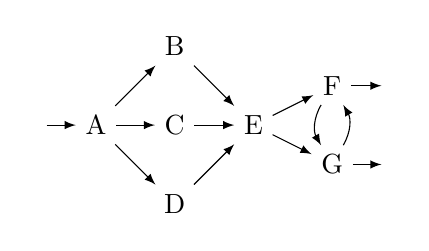
\begin{tikzpicture}
\node[](start) at (-0.75,0){};
\node[](A) at (0,0){A};
\node[](B) at ($(A)+(1,1)$){B};
\node[](C) at ($(A)+(1,0)$){C};
\node[](D) at ($(A)+(1,-1)$){D};
\node[](E) at ($(A)+(2,0)$){E};
\node[](F) at ($(A)+(3,0.5)$){F};
\node[](G) at ($(A)+(3,-0.5)$){G};
\node[](endF) at (3.75,0.5){};
\node[](endG) at (3.75,-0.5){};


\path
(start) edge[-latex]node{} (A)
(A) edge[-latex]node{} (B)
(A) edge[-latex]node{} (C)
(A) edge[-latex]node{} (D)
(B) edge[-latex]node{} (E)
(C) edge[-latex]node{} (E)
(D) edge[-latex]node{} (E)
(E) edge[-latex]node{} (F)
(E) edge[-latex]node{} (G)
(F) edge[-latex, bend right]node{} (G)
(G) edge[-latex, bend right]node{} (F)
(F) edge[-latex]node{} (endF)
(G) edge[-latex]node{} (endG);
\end{tikzpicture}
\end{document}